% LaTeX Template for Project Report, Version 1.0

% Created by: Ernest Mwebaze
%Revised by: Azamuke Denish


\documentclass[12pt, a4paper]{article}
\usepackage[pdftex]{graphicx} %for embedding images
\usepackage{url} %for proper url entries
% \usepackage[bookmarks, colorlinks=false, pdfborder={0 0 0}, pdftitle={<pdf title here>}, pdfauthor={<author's name here>}, pdfsubject={<subject here>}, pdfkeywords={<keywords here>}]{hyperref} %for creating links in the pdf version and other additional pdf attributes, no effect on the printed document
%\usepackage[final]{pdfpages} %for embedding another pdf, remove if not required

\begin{document}
%\renewcommand\bibname{References} %Renames "Bibliography" to "References" on ref page

\pagenumbering{roman} %numbering before main content starts
%Include first stuff: title, acknowledgement, dedication, tables, etc
\begin{titlepage}

\begin{center}

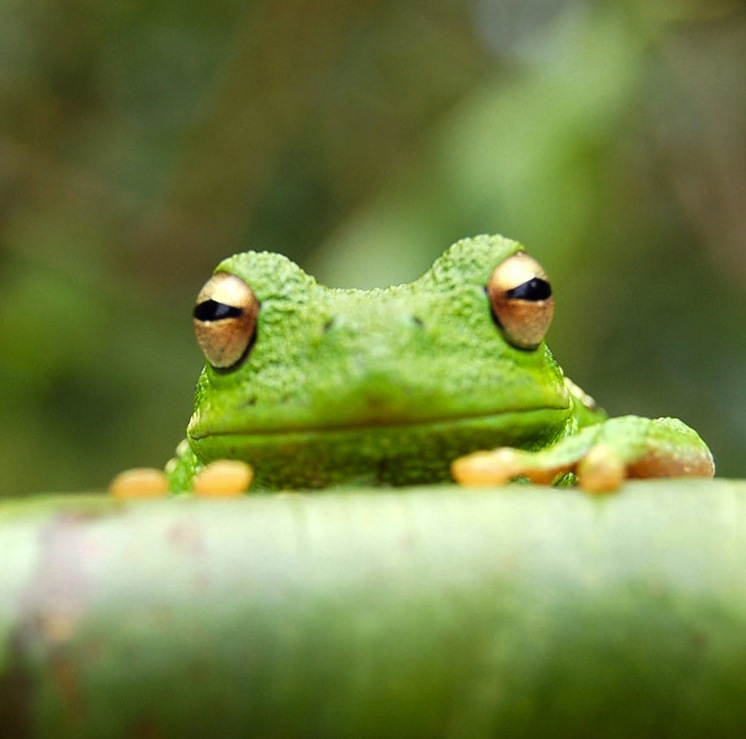
\includegraphics[width=0.2\textwidth]{frog.jpg}\\%\\[0.1in]
\vspace{3em}%
% Title
\Large \textbf {Cybersecurity deepfake placeholder}\\%\\[0.5in]
\vspace{1em}%
\normalsize by \\%
\vspace{1em}
\textup{\small {\bf Giorgio Mocci \\ Marco Motamed}\\}
 \vspace{1em}%
{\bf Laurea Magistrale in Ingegneria Informatica \\ Cybersecurity M}\\[0.5in]

\emph{\textbf{ABSTRACT} \\  A Project Report Submitted to the \\School of Computing and Informatics Technology
for the Study Leading to\\ a Project Report in Partial Fulfilment of the
requirements for the\\ Award of the Degree of Bachelor of Science in \\Computer Science
of Makerere University}

       % \small \emph{Submitted in partial fulfillment of\\
       %  the requirements for the award of the degree of}
        \vspace{1in}

       

% Submitted by
\normalsize {\bf Professore:} \\

[Michele Colajanni]\\
\vspace{1em}

% \begin{table}[h]
% \centering
% \begin{tabular}{lr}\hline \\
% Roll No & Names of Students \\ \\ \hline
% \\
% <Roll no here> & <Name here> \\
% <Roll no here> & <Name here> \\ 
% <Roll no here> & <Name here> \\ \\ \hline 
% \end{tabular}
% \end{table}

% \vspace{.1in}
% \date{}\\
% {\textbf{<Guide's name here>}}\\[0.2in]

\vfill

% Bottom of the page
% \includegraphics[width=0.18\textwidth]{./nitc-logo}\\[0.1in]
% \Large{Department of Computer Science and Engineering}\\
% \normalsize
% \textsc{National Institute of Technology Calicut}\\
% Calicut, Kerala, India -- 673 601 \\
% \vspace{0.2cm}
Dicembre , 2022

\end{center}

\end{titlepage}

\newpage

\section{Introduzione}
%obbiettivo report
Il seguente report ha come obiettivo l'analisi e lo studio dello stato dell'arte relativo alle tecniche, di cybersicurezza, per stabilire l'autenticità di un audio. \\\\
%descrizione tecnologie stato dell'arte 
Tramite l'utilizzo di reti neurali convoluzionali e dell'intelligenza artificiale si è ormai in grado di generare riproduzioni video e/o audio estremamente fedeli alla realtà. Fino a qualche anno fa tali strumenti risultavano essere accessibili solo ad un' "elite" di appassionati e ricercatori con accesso a macchine prestanti e con un'ampia conoscenza dell'argomento. Attualmente, in seguito al boom di queste tecnologie, queste tecniche sono applicabili da chiunque.
\\\\
%impatto sociale relativo
Nonostante queste tecnologie possano essere incredibilmente utili in molti ambiti, ad esempio medico, riabilitativo e sociale, è necessario interrogarsi sui problemi che un utilizzo improprio e scorretto possa causare nella società odierna.\\
Infatti, è possibile sintetizzare delle riproduzioni accurate senza il consenso dell'interessato andando a rubarne l'identità e utilizzandole per fini criminosi.
Queste riproduzioni risultano quasi impossibili da distinguere per l'utente comune e necessitano di ausili tecnologici esterni per essere individuate. \\
Per queste ragioni negli ultimi anni sono nati diversi modelli che, sfruttando il machine learning e l'intelligenza artificiale, permettono di riconoscere e una riproduzione generata artificialmente. 
\\\\
%Come è strutturato il report
Il documento è diviso in tre sezioni sintetizzati come di seguito: 
\begin{enumerate}
    \item Che cos'è un deepfake? Problemi nella società moderna
    \item Come individuare un deepfake (casi studio)
    \item Sperimentazione e lavoro svolto
\end{enumerate}


\pagenumbering{arabic} %reset numbering to normal for the main content

\end{document}
